% ----------------------------------
% 1-Preambulo.
% ----------------------------------
\documentclass[12pt,a4paper]{article}
\usepackage[spanish]{babel}
\usepackage[T1]{fontenc}
\usepackage{textcomp}
\usepackage{lmodern}
\usepackage[utf8]{inputenc}
\usepackage{graphicx}
\usepackage[procnames]{listings} 	%Para escribir códigos.
\usepackage[none]{hyphenat}         %Para no recortar las palabras con guión.
% OJO: se agregaron procnames para usarlos en Python (VER).

\usepackage[bottom]{footmisc} 	 	%Para poner las footnote al final de cada página.
\usepackage[hidelinks]{hyperref} 	%Para que el indice pueda ser linkeado.
\usepackage{amssymb}			 	%Para ecuaciones matemáticas.
\usepackage{amsmath}				%Para matrices.
\usepackage{mathtools}
\usepackage{amsfonts} 
\usepackage{verbatim}				%Para usar comentarios.
\parskip 0.1in 						%Distancia parrafos.

%Biliografías:
%\usepackage[style=authoryear]{biblatex}
%\addbibresource{bibliografias.bib}

\usepackage{float} 							%Para que no se muevan las imágenes de lugar.

\usepackage[
  separate-uncertainty = true,
  multi-part-units = repeat
]{siunitx} 									%Para el \SI del +- .

\usepackage[margin=0.984252in]{geometry} 	%Para los márgenes.
\usepackage{subcaption}
\usepackage{appendix} 						%Para los anexos.

% ----------------------------------
% 1.1-Anexos.
% ----------------------------------

%begin anexos
\makeatletter
\def\@seccntformat#1{\@ifundefined{#1@cntformat}  	%"\@seccntformat" es un comando auxiliar.
   {\csname the#1\endcsname\quad}  					%Default.
   {\csname #1@cntformat\endcsname}					%Enable individual control.
}

\let\oldappendix\appendix 							%Guarda la definicion vigente de \appendix
\renewcommand\appendix{%
    \oldappendix
    \newcommand{\section@cntformat}{\appendixname~\thesection\quad}
}
\makeatother
%\renewcommand{\appendixname}{Anexos}
%\renewcommand{\appendixtocname}{Anexos}
%\renewcommand{\appendixpagename}{Anexos}
%end anexos

% ----------------------------------
% 1.2-Para código Python. 
% ----------------------------------
\usepackage{color}
\definecolor{keywords}{RGB}{255,0,90}
\definecolor{comments}{RGB}{0,0,113}
\definecolor{red}{RGB}{160,0,0}
\definecolor{green}{RGB}{0,150,0}
 
\lstset{language=Python, 
        basicstyle=\ttfamily\small, 
        keywordstyle=\color{keywords},
        commentstyle=\color{comments},
        stringstyle=\color{red},
        showstringspaces=false,
        identifierstyle=\color{green},
        procnamekeys={def,class}}

% ----------------------------------
% 1.3-Índice. 
% ----------------------------------

\setcounter{secnumdepth}{3} 		%Para que ponga 1.1.1.1.
\setcounter{tocdepth}{4} 			%Para que añadir las secciones en el Índice.
\usepackage{chngcntr}				%Para que el número de las figuras esten acordes a la sección.
\counterwithin{figure}{section}

\author{
  Calonge, Federico Matias\\
  \text{calongefederico@gmail.com}
}

\title{
  Tesis \\
  \large Automatización de lectura de Curriculum Vitae  \\
    para selección de personal en el Sector IT}
    
%Para modificar los parrafos y para que se pueda poner subsections:
\makeatletter
\renewcommand\paragraph{\@startsection{paragraph}{4}{\z@}
            {-2.5ex\@plus -1ex \@minus -.25ex}
            {1.25ex \@plus .25ex}
            {\normalfont\normalsize\bfseries}}
\makeatother
\setcounter{secnumdepth}{4} 	%How many sectioning levels to assign numbers to.
\setcounter{tocdepth}{4}    	%How many sectioning levels to show in ToC.
% ----------------------------------
% 2-Documento
% ----------------------------------

\begin{document}

\begin{figure}
  \centering
  
\includegraphics[width=0.2\textwidth]{images/undav-logo.png} 	%Incluyendo logo de la Undav.
  \label{fig:undav-logo}
\end{figure}
\maketitle       		%Para generar el título definido arriba.

\cleardoublepage    %Nueva página

\begin{center}
    \Large
    \vspace{0.9cm}
    \textbf{Resumen}
    
\end{center}

En la Tesis de Ingeniería en Informática que se presenta, se diseña un \textit{sistema de lectura automática de Curriculum Vitae} accesible vía Web. La finalidad del mismo es ayudar al reclutador laboral a elegir a los mejores candidatos para los puestos laborales de IT que tenga disponible. Esta elección se realiza mediante el uso de algoritmos de \textit{machine learning} y basándose, principalmente, en una medición de similitud entre textos: Curriculum Vitae de los candidatos por un lado, y descripciones de los puestos laborales de IT por el otro.
El sistema esta desarrollado utilizando el lenguaje de programación Python, permitiendo verificar la teoría desarrollada.

\begin{center}
    \Large
    \vspace{0.9cm}
    \textbf{Abstract}
\end{center}

This Computer Engineering Thesis introduces an \textit{automatic Curriculum Vitae reading system} accesible via the Web. The purpose of it is to help the job recruiter to choose the best candidates for the available IT job positions. This choice is made through the use of \textit{machine learning} algorithms and based mainly on a measurement of similarity between texts: Curriculum Vitae of the candidates on the one hand, and IT job descriptions on the other hand.
The system is developed using the Python programming language allowing to verify the developed theory.

\cleardoublepage    %Nueva página

\tableofcontents 	%Para insertar el índice general.

\cleardoublepage    %Nueva página

\section{Introducción.}
Los procesos de \textit{reclutamiento y selección laboral} se han vuelto cruciales para el manejo de recursos humanos en el mundo moderno. Con las transformaciones digitales de las empresas y del mercado laboral en general, identificar los perfiles más acordes a las necesidades de la empresa se convirtió en uno de los retos más ambiciosos de Recursos Humanos, en especial cuando hablamos del \textit{Sector IT}, donde año tras año se van generando nuevos puestos de trabajo y estos mismos van creciendo en demanda. Este crecimiento de la demanda en distintos puestos del Sector IT lo podemos evidenciar, a modo de resumen, en la figura \ref{fig:Increasing_Jobs}.

En estos últimos años se implementaron una gran cantidad de herramientas de Software que utilizan algoritmos inteligentes y que permiten automatizar y gestionar información de los candidatos de una manera mucho más intuitiva \cite{trabajos_relacionados_1}\cite{trabajos_relacionados_2}\cite{trabajos_relacionados_3}\cite{trabajos_relacionados_4}\cite{trabajos_relacionados_5}\cite{trabajos_relacionados_6}\cite{trabajos_relacionados_7}\cite{trabajos_relacionados_8}\cite{trabajos_relacionados_9}\cite{trabajos_relacionados_10}\cite{trabajos_relacionados_11} \cite{trabajos_relacionados_12}\cite{trabajos_relacionados_13}\cite{trabajos_relacionados_14}\cite{trabajos_relacionados_15}. La \textit{automatización} se transformó en un factor clave e indispensable para que el reclutador pueda conseguir a los candidatos más relevantes para los puestos que ofrece la empresa en un tiempo muy corto.
Se espera que para el año 2025 muchas tareas realizadas actualmente por humanos, sean automatizadas por máquinas: esto lo podemos evidenciar en la figura \ref{fig:Automatizacion}.

\begin{figure}[H]    %[H] es para que se ubique justo debajo del texto anterior. 
  \centering
  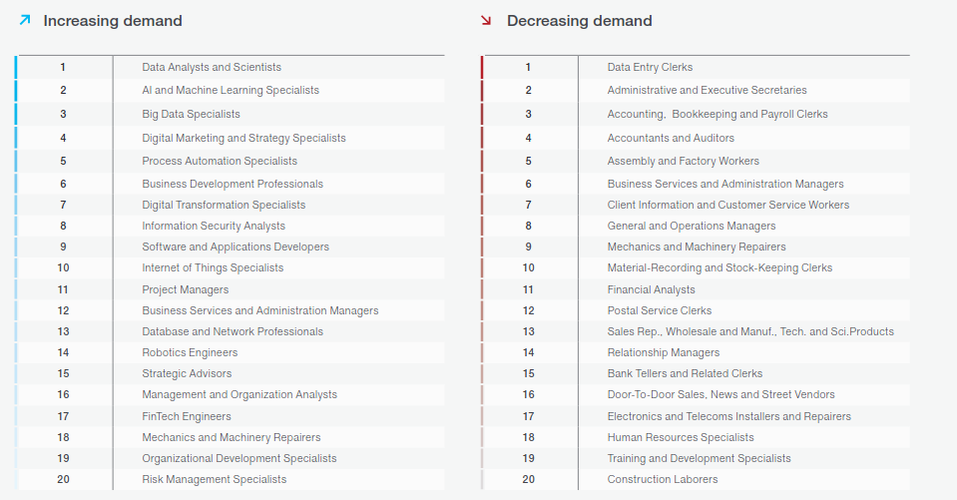
\includegraphics[width=1\textwidth]{images/Increasing_Jobs.png} 	%Incluyendo imagen Flow Core.
  \caption{Top 20 demanda de roles laborales en aumento y disminución para el año 2020, por participación de las empresas encuestadas por el \textit{Foro Económico Mundial}\cite{jobs_future}.}  
  \label{fig:Increasing_Jobs}
\end{figure}

\begin{figure}[H]    %[H] es para que se ubique justo debajo del texto anterior. 
  \centering
  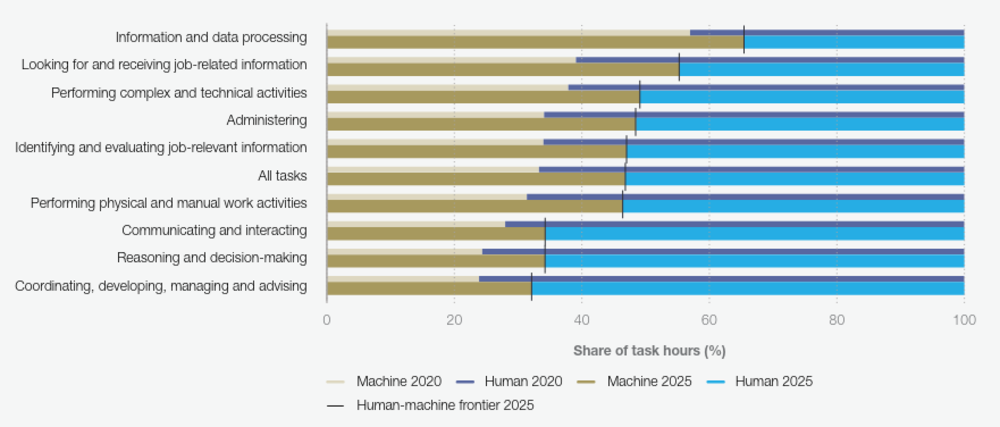
\includegraphics[width=1\textwidth]{images/Automatizacion.png} 	%Incluyendo imagen Flow Core.
  \caption{Porcentaje de tareas realizadas por humanos frente a máquinas, 2020 y 2025 (previsto),
por participación de las empresas encuestadas por el \textit{Foro Económico Mundial}\cite{jobs_future}.}  
  \label{fig:Automatizacion}
\end{figure}

El tema de este Proyecto de Tesis será desarrollar un \textit{sistema de lectura automática de Curriculum Vitae} accesible vía Web. La finalidad del mismo es ayudar al reclutador laboral a elegir a los mejores candidatos para los puestos laborales de IT que tenga disponible. Esta elección se realiza mediante el uso de algoritmos de Machine Learning y basándose, principalmente, en una medición de similitud entre textos: Curriculum Vitae de los candidatos por un lado, y descripciones de los puestos laborales de IT por el otro.

La medición de similitudes de documentos es uno de los problemas más cruciales del \textit{Procesamiento del Lenguaje Natural (NLP)}. Encontrar similitudes entre documentos se utiliza en varios dominios, tales como recomendación de películas, libros o artículos similares, identificación de documentos plagiados o documentos legales, etc. 

Para que las máquinas puedan descubrir esta similitud entre documentos, se necesita definir una forma de medir matemáticamente la similitud, la cual debe ser comparable para que la máquina pueda identificar qué documentos son más similares (o menos). Previamente a esto necesitamos representar el texto de los documentos en una forma cuantificable (que suele ser en forma vectorial), de modo que podamos realizar cálculos de similitud sobre él.

Por lo tanto, los pasos necesarios para que las máquinas puedan medir la similitud entre documentos son:
\begin{enumerate}
\item Convertir un documento en un objeto matemático (vector).
\item Definir y emplear una medida de similitud.
\end{enumerate}

\cleardoublepage    %Nueva página

Para el primer paso se utilizarán los algoritmos de vectorización \textbf{TF-IDF} y \textbf{Word Embeddings}; y para el segundo paso se emplearán las técnicas \textbf{Cosine Similarity} y \textbf{Word Mover's Distance -WMD-}.

Una vez obtenidas estas mediciones de similitud entre los Curriculum Vitae de los candidatos y las descripciones de los puestos laborales de IT, estos valores se utilizarán para alimentar un \textbf{algoritmo de clustering K-means} que a su vez, con sus datos de salida (4 clusters), alimentará a un \textbf{modelo de clasificación KNN}. Finalmente este modelo KNN nos servirá para lograr, en base a los valores de similitud de nuevos candidatos, clasificar qué tan similares son dichos candidatos con respecto a la descripción de un puesto de IT: similitud escasa, similitud media, similitud alta, similitud muy alta.

\cleardoublepage    %Nueva página

\subsection{Objetivos del Proyecto.}

\subsubsection{Objetivo general.}

El objetivo de este Proyecto de Tesis es lograr un desarrollo, tanto teórico como práctico, de un \textit{sistema de lectura automática de Curriculum Vitae} accesible vía Web. La finalidad del mismo es ayudar al reclutador laboral a elegir a los mejores candidatos para los puestos laborales de IT que tenga disponible. Esta elección se realiza mediante el uso de algoritmos de Machine Learning y basándose, principalmente, en una medición de similitud entre textos:  
\begin{itemize}
\item los Curriculum Vitae de los candidatos por un lado, 
\item y descripciones de los puestos laborales de IT por el otro.
\end{itemize} 

\subsubsection{Objetivos específicos.}
Los objetivos específicos de este Proyecto de Tesis son:
\begin{itemize}
\item Describir el estado del arte actual de los Sistemas de lectura y análisis de Curriculum Vitae en las fases de reclutamiento y selección laboral. 
\item Implementar un Sistema de lectura automática de Curriculum Vitae basado en la comparación y medición de similitudes entre textos, para finalmente obtener una visualización de los mejores candidatos para un puesto laboral de IT determinado.  
\item Aprender los conceptos y técnicas principales utilizadas dentro del procesamiento de lenguaje natural (NLP) aplicando técnicas de preprocesamiento y limpieza de textos.
\item Implementar diferentes técnicas para medir similitudes entre los textos (Cosine Similarity y  Word Mover's Distance -WMD-) y diferentes algoritmos de vectorización (TF-IDF y Word Embeddings), analizando su funcionamiento tanto teórica como matemáticamente, ventajas y desventajas.
\item Conocer, implementar e integrar el algoritmo de clustering K-means junto al algoritmo de clasificación KNN para obtener un modelo de clasificación de candidatos en base a las medidas de similitud entre los textos.
\item Evaluar los Frameworks disponibles para tener una UI \footnote{La interfaz de usuario o user inteface (UI) de una página web refiere a todo aquello tangible con lo que los usuarios interactúan de forma directa en la misma.} accesible vía web e integrar el mismo al Sistema.
\item Almacenar datos de candidatos, reclutadores y puestos laborales en una base de datos.
\end{itemize} 

\cleardoublepage    %Nueva página

\subsection{Alcance del Proyecto.}
El alcance de esta Tesis de Grado de Ingeniería incluye el desarrollo de conceptos de análisis de datos y machine learning, procesamiento de lenguaje natural, técnicas de preprocesamiento y limpieza de los datos, algoritmos de vectorización y técnicas para medir la similitud entre textos, algoritmos de clasificación y clustering, integración con frameworks, visualización de datos, y gestión de Base de Datos, de acuerdo a lo enunciado en los objetivos específicos.

\subsection{Organización.}
Este Proyecto de Tesis fue organizado para trabajarlo en tres secciones:

\begin{enumerate}
\item Análisis e investigación inicial. 

Esta sección abarca principalmente la parte teórica del trabajo, haciendo hincapié en el análisis e investigación de:
\begin{itemize}
	\item El estado del arte (actual y pasado) de los sistemas de lectura y análisis de Curriculum Vitae.
	\item Técnicas usadas para el procesamiento del lenguaje natural (NLP).
	\item Técnicas para medir similitudes entre textos: Cosine Similarity y WMD.
	\item Algoritmos de Vectorización: TF-IDF y Word Embeddings.
	\item Algoritmos de Machine Learning para tareas de clasificación (KNN) y clustering (K-means).
\end{itemize} 

Esta primera sección abarca los capítulos \textit{\nameref{2.ReclutamientolaboralenIT}}, \textit{\nameref{3.AlgoritmosdeMachineLearning}} y \textit{\nameref{4.NaturalLanguageProcessing}} de este Informe de Tesis. \\

\item Investigación e implementación de distintas técnicas y algoritmos para la obtención del modelo de clasificación KNN. 

Esta sección hace referencia a la aplicación práctica dentro del marco teórico desarrollado en la primera sección, mediante la realización de una serie de análisis en documentos de Jupyter Notebook \footnote{Aplicación cliente-servidor que permite crear documentos web en formato JSON que siguen un esquema versionado y una lista ordenada de celdas de entrada y de salida. Estas celdas albergan, entre otras cosas, código, texto (en formato Markdown), fórmulas y ecuaciones matemáticas. Estos documentos que se generan funcionan en cualquier navegador estándar.} utilizando Python \footnote{Lenguaje de programación interpretado y multiplataforma de código abierto, popularizado en los últimos años por su facilidad para trabajar con inteligencia artificial, big data, machine learning y data science, entre muchos otros campos en auge.}, para la obtención final de nuestro modelo de clasificación KNN capaz de clasificar, en base a los valores de similitud de nuevos candidatos, qué tan similares son dichos candidatos con respecto a la descripción de un puesto de IT: similitud escasa, similitud media, similitud alta, similitud muy alta. 

\cleardoublepage    %Nueva página

Los items que abarca esta sección son:

\begin{itemize}
	\item Obtención de sets de datos: curriculums vitae y descripciones laborales. 
	\item Preprocesamiento de los textos.
	\item Comparación entre textos y obtención de similitudes entre los mismos mediante el uso de las técnicas para medir distancias y obtener dichas similitudes (WMD y Cosine Similarity) y los algoritmos de vectorización (TF-IDF y Word Embeddings).
	\item Obtención del modelo de clasificación KNN utilizando como datos de entrada los clusters devueltos por el algoritmo K-means obtenidos en base a las mediciones de similitud previamente realizadas.
	\item Análisis y primeras visualizaciones de los resultados.
\end{itemize} 
 
Esta sección abarca el capítulo \textit{\nameref{5.Implementacion}} (desde \textit{\nameref{5.1.Obtenciondelmodelopredictivo}} hasta \textit{\nameref{5.4.Predicciondenuevasmuestrasyresultadosobtenidos}}) de este Informe de Tesis. \\

\item Investigación e integración al sistema web.

Esta última sección hace referencia a la reutilización de las funciones que contenian la lógica de los distintos algoritmos utilizados junto con el modelo de clasificación KNN obtenidos previamente en la sección 2, para integrar todo esto en el sistema Web que, a su vez, esta integrado a una base de datos relacional. De esta manera, el sistema cuenta con una interfaz gráfica permitiendo interactuar entre candidatos y reclutadores y, principalmente, permitiendo que el reclutador sea capaz de obtener un listado con los N candidatos más similes a un puesto determinado, y ordenados de mayor a menor de acuerdo a esta \textit{similitud}. Dicha \textit{similitud} representa el resultado obtenido de la clasificación por nuestro modelo KNN. 

Los items principales de esta sección son:
\begin{itemize}
	\item Definición de los usuarios que accederán al sistema.
	\item Definición de los datos que se almacenarán.
	\item Integración de frameworks y bases de datos.  
	\item Modelado, filtrado y visualización de los datos.
	\item Reutilización e integración al sistema de los algoritmos y del modelo KNN utilizados en la fase previa.	
	\item Evaluación del funcionamiento de todo el Sistema integrado.
\end{itemize} 

Esta última sección abarca el capítulo \textit{\nameref{5.Implementacion}} (desde \textit{\nameref{5.5.IntegracionalSistemaWeb}} hasta el final del capítulo) de este Informe de Tesis.
\end{enumerate}

\cleardoublepage    %Nueva página

\section{Reclutamiento y selección laboral.}\label{2.ReclutamientolaboralenIT}

En este capítulo se va a realizar una introducción a los procesos de reclutamiento y selección laboral, sus diferencias y diferentes tareas involucradas. Por último, se llevará a cabo un análisis del Estado de Arte actual de los sistemas de cribado (o más conocidos como sistemas de \textit{screening}) y se detallará el enfoque utilizado para este Proyecto.

\subsection{Introducción.}

Los procesos de \textit{reclutamiento y selección laboral} se han vuelto cruciales para el manejo de recursos humanos en el mundo moderno. Con las transformaciones digitales de las empresas y del mercado laboral en general, identificar los perfiles más acordes a las necesidades de la empresa se convirtió en uno de los retos más ambiciosos de Recursos Humanos, en especial cuando hablamos del \textit{Sector IT}, donde año tras año se van generando nuevos puestos de trabajo y estos mismos van creciendo en demanda. 

Los \textit{reclutadores}, dentro de un departamento de recursos humanos, son los encargados de llevar a cabo los procesos de \textit{reclutamiento} y \textit{selección} laboral. Uno de sus objetivos principales es buscar talento humano para cubrir los puestos de trabajo vacantes que tenga la empresa.

\subsection{Reclutamiento vs selección.}\label{SeleccionYReclutamiento}

El \textbf{reclutamiento} es el proceso de atracción, búsqueda, recolección e identificación de candidatos que encajan con la oferta de trabajo y, en definitiva, con la empresa. El objetivo del reclutamiento es \textit{atraer}, \textit{buscar} e \textit{identificar} a los candidatos más adecuados y mejor calificados para el puesto disponible, según las necesidades de la empresa\cite{seleccion_reclutamiento_2}. 

El proceso de reclutamiento incluye las siguientes actividades:
\begin{itemize}
\item Identificación de las necesidades del puesto a cubrir. 
\item Análisis de la descripción y especificaciones del puesto.
\item Identificación de posibles fuentes de candidatos cualificados para el puesto.
\item Publicacion del puesto vacante en dichas fuentes.
\item Atracción de candidatos para aplicar al puesto.
\item Manejo apropiado en las respuestas y en los escrutinios a las postulaciones.
\end{itemize}

\cleardoublepage    %Nueva página

En cambio, la \textbf{selección} es un proceso posterior al reclutamiento, donde se evalua más detalladamente y se entrevista a los candidatos para el trabajo en particular. El objetivo de la selección es \textit{elegir} y \textit{hacer efectiva la contratación} del candidato más adecuado y mejor calificado para el puesto disponible, según las necesidades de la empresa. Este procedimiento particiona a los candidatos en dos secciones: a los que se les ofrecerán el trabajo, y a los que se descartarán\cite{seleccion_reclutamiento_2}.

El proceso de selección incluye las siguientes actividades: 
\begin{itemize}
\item Recepción de la aplicación al puesto.
\item Cribado o Screening de los candidatos, lo que permite avanzar con los candidatos adecuados y descartar a los no adecuados para el puesto.
\item Entrevistas a los candidatos.
\item Manejo de tests a los candidatos, tales como tests médicos o psicológicos. 
\item Manejo de exámenes a los candidatos, tales como exámenes técnicos, de aptitud, inteligencia, performance, etc.
\item Evaluación de las referencias de los candidatos.
\item Decisión final acerca de la contratación o no contratación del candidato.
\end{itemize}

Como conclusión, podemos decir que en la fase de \textbf{reclutamiento} se trata de encontrar muchos candidatos que cumplan con los requisitos de la oferta; mientras que en la etapa de \textbf{selección} se debe elegir al mejor candidato para las necesidades de la empresa. 

\cleardoublepage    %Nueva página

\subsection{Evolución de los procesos de reclutamiento y selección laboral.}
Los procesos de reclutamiento y selección laboral fueron evolucionando a lo largo del tiempo\cite{trabajos_relacionados_10}:

En los modelos de reclutamiento y selección de \textbf{primera generación}, las empresas anunciaban sus vacantes de puestos laborales en diarios, revistas, radio y en televisión. Los candidatos enviaban sus currículums por correo postal y los mismos se clasificaban manualmente: algo muy tedioso y que llevaba mucho tiempo en realizar. Una vez \\ preseleccionados los candidatos, los reclutadores llamaban a los mismos para realizar las rondas de entrevistas. 

Luego pasamos a la \textbf{segunda generación}. En esta época las empresas comenzaron a crecer y también lo hicieron las necesidades de reclutamiento y selección. Las empresas empezaron a subcontratar sus procesos de reclutamiento y selección, naciendo de esta manera las consultoras o agencias de contratación. Estas consultoras requerían que los candidatos cargaran sus currículums en sus sitios web en formatos particulares. Luego, las consultoras revisaban los datos de los candidatos y preseleccionaban a los mismos para la empresa. El gran inconveniente de este proceso fue que habían numerosas consultoras y cada una tenía su propia y única forma de selección, no era un proceso uniforme.

Para intentar superar los problemas anteriores, se llegó a una \textbf{tercera generación}, en la que estamos actualmente. En esta generación se crearon, y siguen creándose, una gran cantidad de herramientas de Software que utilizan algoritmos inteligentes y permiten automatizar y gestionar información de los candidatos de una manera mucho más intuitiva. Estos sistemas ayudan a los reclutadores dentro de las empresas y consultoras a analizar la información de cualquier Curriculum Vitae y clasificarlos o listarlos en función de los puestos disponibles. De esta manera, cuando el reclutador publica una oferta de trabajo, estos sistemas clasifican o listan a los currículums basándose en distintas métricas (por ejemplo palabras clave) mostrando así los candidatos más relevantes para la empresa o consultora.

\cleardoublepage    %Nueva página

\subsection{Cribado o screening.}  

Como vimos anteriormente en \textit{\nameref{SeleccionYReclutamiento}}, el screening (o tambien conocido como cribado) es una etapa del proceso de selección. 
En esta etapa los reclutadores revisan los Currículums Vitae que fueron recibiendo por parte de los candidatos, y \\ preseleccionan a los que mejor se adapten a los requisitos de la oferta de empleo de la empresa. Este proceso es muy importante dentro del proceso de selección, ya que permite valorar en ese momento si el candidato es apto para continuar en el proceso de selección o, en caso contrario, si el mismo se descarta por no considerarlo adecuado para el puesto.

\subsubsection{Screening manual vs screening automatizado}  

Si el proceso de screening sigue el modelo tradicional y se realiza manualmente, es un proceso muy tedioso y que lleva mucho tiempo por parte del reclutador, el cual tiene que evaluar una gran cantidad de Curriculums Vitae. Existe un estudio\cite{estudio_eye_tracking} relizado en 2018 por Ladders Inc., empresa lider en sitios de carrera, donde se estudió cuánto tiempo en promedio tarda un reclutador en dar una primera vista rápida a un Curriculum Vitae de un candidato. Se descubrió que este tiempo es, en promedio, de 7.4 segundos. Este es el tiempo en el que el reclutador decide inicialmente si el candidato sigue (o no) con el proceso de selección.

Sin embargo, este tiempo es engañoso: ya que este estudio fue realizado con la aplicación de muchos Curriculums vitae que no cumplian con los criterios mínimos para calificar a los puestos; es por esto que los reclutadores realizaban una primer vista rápida y los descartaban (o no) a los pocos segundos. Si las aplicaciones provenieran de Curriculums Vitae que cumplan con los requisitos mínimos del puesto, este tiempo de observación sería mucho mayor, ya que el reclutador examinaría con mayor detalle los curriculums.

Adicionalmente, este estudio tampoco tiene en cuenta el tiempo consumido por el reclutador al comparar el Curriculum Vitae del candidato con la descripción o requisitos del puesto laboral, por lo que el tiempo en realizar un screening manual se incrementaría significativamente.

Otra de las desventajas al considerar el screening como un proceso manual, es que muchos son los factores que pueden influir al reclutador en el momento de tomar la decisión de descarte o selección del candidato, ya sea cansancio por el volumen de los curriculums ya revisados, la estructura, elementos discriminatorios o información incompleta dentro de los mismos, etc. Es por esto que las probabilidades de descartar prematuramente a un candidato válido son muy altas.

Frente a estas desventajas del modelo tradicional y poco eficiente del screening manual existe una solución: la \textit{automatización}. Actualmente existen sistemas automatizados y basados en Inteligencia Artificial que permiten realizar el screening de un volumen importante de curriculums en unos pocos segundos (Ver \textit{\nameref{Estado_del_arte}}). De esta manera, el proceso de screening no estaría afectado a factores externos que puedan influir en la decisión del reclutador, y además la herramienta sería capaz de entregar un listado justificado de los mejores candidatos para la siguiente fase del proceso en un tiempo relativamente corto.

\cleardoublepage    %Nueva página

Uno de los beneficios potenciales de utilizar sistemas automatizados e inteligentes en los procesos de screening es el acortamiento de los ciclos de contratación, lo que hace que la organización responda mejor a los solicitantes y sea más capaz de competir con otras organizaciones por los mejores candidatos\cite{seleccion_reclutamiento_1}.  

Muchos gerentes de recursos humanos depositan sus esperanzas en la tecnología y las herramientas automatizadas e inteligentes: desde el aumento de la eficiencia y la reducción de costos hasta el aumento de las aplicaciones de candidatos y la estandarización de todos sus sistemas de selección\cite{seleccion_reclutamiento_1}.

\subsection{Sistemas de screening: Estado del arte.}\label{Estado_del_arte}

Tal como mencionamos en la sección anterior, un sistema de screening automatizado e inteligente nos permite entregar al reclutador una shortlist con los candidatos que mejor se adaptan a los requisitos de la oferta de empleo de la empresa. De esta manera, al realizar dicha preselección de candidatos, el reclutador podrá seguir con las etapas posteriores de selección o podrá realizar otro screening manual para descartar a otros candidatos.

A continuación detallaremos una serie de trabajos de relevancia (tanto de implementación como de investigación) donde se utilizaron distintos enfoques para desarrollar o sugerir un desarrollo de un sistema de screening de candidatos.

En \cite{trabajos_relacionados_1} utilizaron el \textit{algoritmo KNN} para clasificar los curriculums de los candidatos en diferentes categorías, y luego utilizaron la métrica de similitud \textit{Cosine Similarity} para averiguar qué tan cerca está el curriculum del candidato con respecto a la descripción de los puestos, y realizar un ranking acorde a estos resultados.

En \cite{trabajos_relacionados_2} utilizaron una herramienta inteligente llamada \textit{EXPERT mapping-based candidate screening} que utiliza  \textit{ontology mapping}\footnote{La \textit{ontología (ontology)} permite la especificación explícita de un dominio de discurso, que permite acceder y razonar sobre el conocimiento de un agente. Las ontologías elevan el nivel de especificación del conocimiento, incorporando semántica a los datos.
El \textit{mapeo de ontologías (ontology mapping)} es el proceso mediante el cual dos ontologías se relacionan semánticamente a nivel conceptual y las instancias de ontología de origen se transforman en entidades de ontología de destino de acuerdo con esas relaciones semánticas.\cite{ontology_mapping} } para crear un sistema automatizado para el screening inteligente de candidatos. 

En \cite{trabajos_relacionados_3} y \cite{trabajos_relacionados_4} también se utilizan sistemas basados en \textit{ontologías} para extraer datos de curriculums y realizar macheos con los puestos disponibles.

En \cite{trabajos_relacionados_5} sugieren un método de matching basado en un \textit{modelo probabilístico} para ser utilizado en la selección y recomendación de candidatos. 

En \cite{trabajos_relacionados_6} se propuso un aistema automatizado de screening de currículums que usa \textit{Vector Space Model}\footnote{Modelo algebraico para representar documentos de textos en lenguaje natural de una manera formal mediante el uso de vectores de identificadores. Es utilizado para la recuperación, filtrado, indexado y cálculo de relevancia de información.} para machear cada curriculum con la descripción del puesto correspondiente y \textit{cosine similarity} como medida de similitud.

\cleardoublepage    %Nueva página

En \cite{trabajos_relacionados_7} y \cite{trabajos_relacionados_8} se propuso un sistema para el screening de candidatos, para el cual se utiliza \textit{cosine similarity}, \textit{KNN} y un \textit{sistema de recomendación basado en contenido (Content Based Filtering, CBF)} para buscar los curriculums más cercanos a la descripción del puesto.

En \cite{trabajos_relacionados_9} se propuso un sistema para el ordenamiento y clasificación de currículums utilizando el concepto de inteligencia artificial (sin especificar qué algoritmos o técnicas específicas se deberían usar). Lo que se propuso fue un esquema de trabajo para luego seguir con la implementación del sistema; el cual permitiría clasificar a todos los currículums de acuerdo con los requisitos de la empresa y los enviaría a Recursos Humanos para su posterior consideración.

En \cite{trabajos_relacionados_10} se diseñó un sistema que ayuda a los reclutadores a seleccionar los curriculums basados en la descripción del trabajo. Ayuda en un proceso de contratación fácil y eficiente al extraer los requisitos automáticamente. Este sistema utiliza un \textit{modelo NER (Named entity recognition)} \footnote{Subtarea de \textit{information extraction (IE)} que permite buscar y categorizar entidades específicas en un cuerpo o cuerpos de textos.}.

En \cite{trabajos_relacionados_11} y \cite{trabajos_relacionados_12} se implementan sistemas basados en \textit{semantic anotation}\footnote{Proceso de etiquetado de documentos con conceptos relevantes. Los documentos se enriquecen con metadatos que permiten vincular el contenido a los conceptos, descritos en un gráfico de conocimiento. Esto hace que el contenido no estructurado sea más fácil de encontrar, interpretar y reutilizar.} y \textit{ontologías}, permitiendo realizar macheos entre las ofertas de trabajo y los curriculums de los candidatos.

En \cite{trabajos_relacionados_13} se utiliza \textit{relevance feedback}\footnote{Característica de algunos sistemas de \textit{information retrieval (IR)}. La idea de relevance feedback es tomar los resultados que se devuelven inicialmente de una consulta/query determinada, recopilar los comentarios de los usuarios y usar información para evaluar si esos resultados son relevantes o no para realizar una nueva consulta/query.} para la implementación de un sistemas que intenta encontrar a los mejores candidatos para las distintas ofertas de trabajo.

\textit{Paul Resnick} y \textit{Hal R. Varian} fueron pioneros en los \textit{sistemas de recomendación}\footnote{Un \textit{sistema de recomendación} es una subclase de los sistemas de \textit{Information filtering (IF)} que busca predecir la calificación o la preferencia que un usuario le puede dar a un artículo. En palabras simples, es un algoritmo que sugiere artículos relevantes para los usuarios.}\cite{sistema_recomendacion}.
En \cite{trabajos_relacionados_14} y \cite{trabajos_relacionados_15} se utilizaron dichos \textit{sistemas de recomendación} junto a otros algoritmos para implementar aplicaciones de screening y clasificación de candidatos. Esto es debido a que, dado que el perfil del candidato es necesario para un puesto en particular, la forma en que se comparan los curriculums de los candidatos es muy similar a un sistema de recomendación. 

\cleardoublepage    %Nueva página

\subsection{Enfoque del Proyecto.}

Como vimos en la sección anterior, hay cientos de enfoques y combinaciones posibles para realizar un sistema de screening automático e inteligente.

El enfoque elegido para este Proyecto de Tesis fue realizar un sistema híbrido que utilice técnicas de mediciones de similitud entre los curriculums de los candidatos y las descripciones de los puestos disponibles, junto con técnicas de machine learning (de clustering y clasificación). 

Como métricas de medición de similitud se utilizó una de las más comúnmente usadas, \textit{similitud del coseno}, y una métrica que \textbf{no se usó en ninguno de los trabajos anteriores} pero, que sin embargo, es muy reciente y prometedora, y es la principal técnica utilizada para la medición semántica de la distancia entre textos, \textit{Word Mover's Distance (WMD)}. Estas métricas serán explicadas más en detalle en las secciones posteriores (Ver \nameref{Tecnicas_Simil_textos}).

Una vez utilizadas estas mediciones de similitud se utilizaron algoritmos de machine learning: un algoritmo de clustering (K-means), y luego un modelo de clasificación KNN. 

Además del uso de \textit{Word Mover's Distance}, otro aspecto distintivo de este sistema es que se realizó una \textbf{integración a una interfaz web}, la cual la mayoría de los sistemas descriptos anteriormente no poseen. De esta manera, mediante la interfaz web se logra una interacción entre usuarios candidatos y reclutadores y, principalmente, permite que el reclutador sea capaz de visualizar un listado con los N candidatos más similes a un puesto determinado.

Por último, cabe destacar que los trabajos anteriormente mencionados no tienen un fácil acceso a los datasets ni al código que utilizaron para dichos sistemas, por lo que seguir el trabajo de ellos aplicando las mejoras que mencionan en sus artículos es una tarea casi imposible. En cambio, \textbf{este sistema será de código abierto}: los datasets, modelos y códigos utilizados estarán disponibles en Github y Git LFS\footnote{\url{https://github.com/FedericoCalonge/automatic_reading_of_CVs_using_text_similarity}}.

\cleardoublepage    %Nueva página\\

\section{Algoritmos de Machine Learning.}\label{3.AlgoritmosdeMachineLearning}

Para comenzar el marco teórico de esta tesis, es necesario explicar qué es Machine Learning y cómo se pueden clasificar a los distintos algoritmos según su tipo de aprendizaje. 
En este capítulo se va a explicar el objetivo del aprendizaje supervisado y no supervisado en Machine Learning haciendo énfasis en los algoritmos K-Nearest Neighbor (KNN) y K-means.

\subsection{Introducción.}
\colorbox{red}{FALTA}
Los métodos que utilizaremos en este Proyecto de Tesis serán...

\subsection{K-Nearest Neighbor (KNN).}
\colorbox{red}{FALTA}
K-Nearest Neighbor (o K Vecinos más Próximos en español), blablabal....

\cleardoublepage

\subsection{K-Means.}
\colorbox{red}{FALTA}
K-Means (o K-Medias en español), blablaba...

\cleardoublepage

\subsubsection{Elbow Method.}
\colorbox{red}{FALTA}
Elbow Method (o Método del codo en español), blablaba...

\cleardoublepage

\section{Natural Language Processing.}\label{4.NaturalLanguageProcessing}

\colorbox{red}{FALTA}

\cleardoublepage

\subsection{Introducción.}
\colorbox{red}{FALTA}

\cleardoublepage

\subsection{Preprocesamiento de textos.}
\colorbox{red}{FALTA}

\cleardoublepage

\subsection{Similitud entre textos.}
\colorbox{red}{FALTA}

\cleardoublepage

\subsection{Técnicas para medir Similitud entre textos.}\label{Tecnicas_Simil_textos}
\colorbox{red}{FALTA}

\subsubsection{Cosine Similarity.}
\colorbox{red}{FALTA}

Cosine Similarity se basa en la medición del coseno del ángulo entre dos vectores proyectados en un espacio multidimensional para lograr medir la similitud de los documentos (un menor ángulo indica una mayor similitud). En este contexto, estos dos vectores representan matrices que contienen el recuento de palabras de dos documentos. Una de sus limitaciones es que  no tiene la habilidad de reconocer si las palabras que compara son semánticamente similares.

\cleardoublepage

\subsubsection{Word Mover's Distance (WMD).}
\colorbox{red}{FALTA}

Anteriormente, mencionamos que una de las limitaciones de Cosine Similarity es que no tiene habilidad de reconocer si las palabras que compara son semánticamente similares. En cambio, Word Mover's Distance (WMD) es un algoritmo más complejo que sí permite reconocer las relaciones semánticas; su limitación son las relaciones sintácticas (VER.........). WMD se basa en word embeddings y permite medir la distancia entre documentos (una menor distancia indica una mayor similitud).

\cleardoublepage

\subsection{Algoritmos de vectorización.}
\colorbox{red}{FALTA}

Previamente a utilizar Cosine Similarity y WMD para (-----completar-----) se debe emplear algún algoritmo de vectorización que permita representar las palabras de nuestros textos a un espacio vectorial. De esta forma Cosine Similarity y WMD podrán interpretarlos de la mejor manera. 
Como algoritmos de vectorización se utilizarán TF-IDF y Word Embeddings.

\subsubsection{TF-IDF.}
\colorbox{red}{FALTA}

El algoritmo TF-IDF asigna valores numéricos a las palabras en función de la frecuencia con que aparecen en los textos para medir la frecuencia de ocurrencia de un término en la colección de documentos, expresando  cuán relevante es una palabra para un documento en una colección. 

\cleardoublepage

\subsubsection{Word Embeddings.}
\colorbox{red}{FALTA}

Los Word Embeddings son necesarios para utilizar WMD.
Los Word Embeddings son una de las variantes más populares para representar textos.  Son vectores previamente entrenados y generados mediante un modelo de red neuronal secuencial; de esta manera son capaces de capturar los contextos de una palabra en el documento llegando a poder contener información semántica y sintáctica. 

\cleardoublepage

\paragraph{¿Cómo entrenar Word Embeddings?}
\colorbox{red}{FALTA}

\cleardoublepage

\section{Implementación.}\label{5.Implementacion}

La implementación de este Sistema se trabajó en dos grandes partes:
\begin{enumerate}
\item Obtención del modelo de clasificación. 

En esta primera parte se obtuvieron y preprocesaron datasets de Curriculum Vitae de distintos candidatos y descripciones de puestos de trabajo de IT publicados por distintas empresas, para luego ser comparados y obtener similitudes entre los textos utilizando las técnicas para medir distancias y obtener dichas similitudes (WMD y Cosine Similarity) y los algoritmos de vectorización (TF-IDF y Word Embeddings).

Una vez obtenidas estas mediciones de similitud entre los Curriculum Vitae de los candidatos y las descripciones de los puestos laborales de IT, estos valores se utilizaron para alimentar un algoritmo de clustering K-means que a su vez, con sus datos de salida (4 clusters), alimentan a un modelo de clasificación KNN. Finalmente, con este modelo KNN logramos, en base a los valores de similitud de nuevos candidatos, clasificar qué tan similares son dichos candidatos con respecto a la descripción de un puesto de IT: similitud escasa, similitud media, similitud alta, similitud muy alta.

Estos análisis se realizaron en documentos de Jupyter Notebook utilizando Python; y sirvieron para evaluar el comportamiento del modelo de clasificación y los distintos algoritmos de medición de similitudes para luego ser utilizados en la siguiente etapa. \\

\item Integración al Sistema Web. 

Etapa posterior a la primera parte. Una vez observado que los resultados fueron los esperables, lo que se hizo fue reutilizar las funciones que contenian la lógica de los distintos algoritmos utilizados junto con el modelo de clasificación KNN obtenidos previamente en la parte 1, para integrar todo esto en el sistema Web. Este sistema web está realizado en Django \footnote{Framework de desarrollo web de código abierto, escrito en Python, que respeta el patrón de diseño conocido como modelo–vista–controlador.}, y cuenta con una base de datos relacional que contiene la información de los candidatos y reclutadores junto con los Curiculum Vitae y puestos que hayan cargado. 

De esta manera, nuestro sistema cuenta con una interfaz gráfica permitiendo interactuar entre candidatos y reclutadores y, principalmente, permitiendo que el reclutador sea capaz de obtener un listado con los N candidatos más similes a un puesto determinado, y ordenados de mayor a menor de acuerdo a esta \textit{similitud}. Dicha \textit{similitud} representa el resultado obtenido de la clasificación por nuestro modelo KNN.

\end{enumerate}

\cleardoublepage

\subsection{Obtención del modelo de clasificación.}\label{5.1.Obtenciondelmodelopredictivo}

\subsubsection{Introducción.}
Como inicio definamos qué es un modelo. En nuestro caso, un modelo representa ....
Este modelo se construyó en base a ...
La implementación de este Sistema se realizó en Python...

\subsubsection{Esquema.}
Como podemos ver la figura \ref{fig:FlowCoreSystem} representa el procedimiento utilizado para la obtención de nuestro modelo de clasificación. 

\begin{figure}[H]    %[H] es para que se ubique justo debajo del texto anterior. 
  \centering
  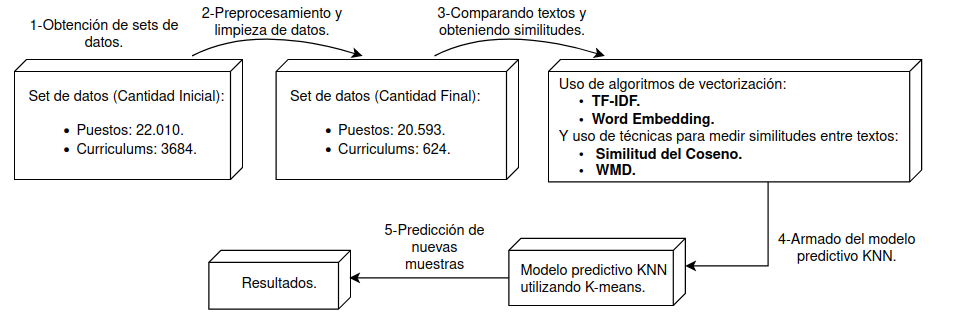
\includegraphics[width=1\textwidth]{images/flow-core.png} 	%Incluyendo imagen Flow Core.
  \caption{Pipeline Flow para la obtención del modelo de clasificación KNN}  
  \label{fig:FlowCoreSystem}
\end{figure}

\cleardoublepage

\subsubsection{Obtención de sets de datos.}
En primer lugar debemos definir qué es un set o conjunto de datos.
Un set o conjunto de datos es una tabla de una base de datos o, matemáticamente, una matriz estadística de datos. Cada columna de la tabla representa una variable del set de datos; y cada fila representa a un miembro determinado del mismo.

Para este Proyecto utilizamos dos grandes sets de datos que se obtuvieron mediante la recolección de distintos archivos alojados en la Web, los cuales estan descriptos a continuación.

\paragraph{Curriculum Vitae.}
Los set de datos de Curriculum Vitae de los candidatos se obtuvieron de las siguientes fuentes:

\begin{enumerate}
\item 228 Curriculums en formato docx y posteriormente convertidos a pdf, obtenidos del sitio Kaggle\footnote{\url{https://www.kaggle.com/palaksood97/resume-dataset}}. Estos pdfs son candidatos de la India con experiencia en el rubro de IT.
\item 2484 Curriculums en formato CSV, obtenidos del sitio Kagle\footnote{\url{https://www.kaggle.com/snehaanbhawal/resume-dataset}}. Este CSV cuenta con curriculums vitae obtenidos del sitio web de postulación de trabajos 'livecareer.com'.
\item 962 Curriculumns en formato CSV, obtenidos del sitio Kaggle\footnote{\url{https://www.kaggle.com/gauravduttakiit/resume-dataset}}. Este CSV cuenta con curriculums vitae repartidos en distintas categorías de IT.
\item 10 Curriculums en formato PDF, los cuales los cuales fueron obtenidos como ejemplos mediante una recolección propia de distintos sitios web. 
\end{enumerate}

\paragraph{Descripciones Puestos Laborales.}

Los set de datos de descripciones de puestos laborales se obtuvieron de las siguientes fuentes:

\begin{enumerate}
\item 22.000 descripciones en formato CSV; obtenido del sitio Kaggle\footnote{\url{https://www.kaggle.com/PromptCloudHQ/us-technology-jobs-on-dicecom}}. El CSV cuenta con descripciones de puestos obtenidos del sitio web de USA de postulación de trabajos del rubro de IT 'Dice.com'.
\item 10 descripciones en formato CSV; obtenidas como ejemplos mediante una recolección propia del sitio Indeed\footnote{\url{https://www.indeed.com/q-USA-jobs.html}} para puestos de trabajo de IT.
\end{enumerate}

\cleardoublepage

\subsubsection{Preprocesamiento y limpieza de datos.}
Previamente a utilizar las técnicas para medir distancias y obtener similitudes entre textos (WMD y Cosine Similarity) y los algoritmos de aprendizaje (KNN y K-Means) necesitamos que los datos que comparemos e introduzcamos en los algoritmos estén lo más limpios posible; ya que de lo contrario las mismos podrían clasificar o predecir de forma errónea. Este análisis previo sobre los datos debe ser minucioso ya que puede haber valores incoherentes o absurdos.

El procedimiento para la Limpieza de los Curriculum Vitae y las descripciones de los puestos laborales fue el siguiente:

\begin{enumerate}
\item Convertimos todo a minúscula.
\item Eliminamos datos no relevantes para nuestros análisis (mails y páginas web).
\item Eliminamos signos de puntuación y caracterés especiales (incluyendo números).
\item Eliminamos stop words.
\item Eliminamos common words no relevantes para nuestros análisis.
\item Aplicamos Lematización y Tokenización.
\item Eliminamos repetidos.
\item Obtenemos y usamos bi-gramas.
\end{enumerate}

Luego de aplicar preprocesamiento y limpieza de datos nos quedarán los siguientes tamaños de nuestros datasets:
\begin{itemize}
\item 624 curriculums vitae de candidatos (en formato pdf y csv).
\item 20593 descripciones de puestos de IT (en formato csv).
\end{itemize}

\cleardoublepage

\subsubsection{Cantidad final del set de datos y su uso en las distintas etapas.}

El total de 624 curriculums vitae de candidatos y 20593 descripciones de duestos de IT que mencionamos previamente, serán utilizados para el entrenamiento y obtención de vectores mediante TF-IDF (para el posterior cálculo de Cosine Similarity) y para el entrenamiento de Word2Vec y obtención de los Word Embeddings (para el posterior cálculo de WMD).

Por otro lado, para calcular Cosine Similarity y WMD, para utilizarlos en K-means y para entrenar a nuestro algoritmo KNN, utilizaremos únicamente una porción de nuestros datasets:

1-Para el cálculo de Cosine Similarity y WMD:
\begin{itemize}
\item 301 curriculums vitae de candidatos.
\item 201 descripciones de puestos de IT.
\end{itemize}
Nota: No obstante, al realizar los cálculos de distancias compararemos cada curriculum vitae con cada Job Description, obteniendo un dataframe total de 3131 filas con sus respectivo valores de WMD y Cosine Sim.

2-Para el uso de K-means y entrenamiento con KNN (eliminamos un curriculum vitae y una descripción de puesto IT que los utilizamos en '3-'):
\begin{itemize}
\item 300 curriculums vitae de candidatos.
\item 200 descripciones de puestos de IT.
\end{itemize}        
Nota: como se comentó previamente, nos quedarán 3000 filas / puntos para usar en K-means y entrenar KNN; llegando a representar estos 3000 puntos en un plano de 2 dimensiones.

3-Para la clasificación de nuevas muestras mediante KNN:
\begin{itemize}
\item 1 curriculum vitae de candidatos.
\item 1 descripción de puesto de IT.
\end{itemize}
Nota: como se comentó previamente, nos quedarán 131 filas para clasificar.

¿Por qué utilizamos solo una porción de nuestros datasets?: Esto es debido a los drawbacks de WMD y KNN.
\begin{itemize}
\item WMD: posee una alta complejidad en el cálculo de la distancia, teniendo un tiempo de ejecución muy elevado. Como ejemplo, al correrlo localmente, el cálculo de WMD para 3131 filas tardó 7 horas; frente a los 3 segundos que tardó el cálculo de Cosine Similarity para la misma cantidad de filas.
\item KNN: KNN es una gran opción para datasets pequeños con pocas variables de entrada; pero tiene problemas cuando la cantidad de entradas es muy grande. Cada variable de entrada puede considerarse una dimensión de un espacio de entrada p-dimensional. En grandes dimensiones, los puntos que pueden ser similares pueden tener distancias muy grandes. Además, cada vez que se va a hacer una predicción con KNN, busca al vecino más cercano en el conjunto de entrenamiento completo. Por esto, se debe utilizar un dataset pequeño para que el clasificador KNN completa su ejecución rápidamente.
\end{itemize}
En conclusión, al utilizar solo una porción de nuestros datasets para obtener los distintos cálculos de distancias y entrenar KNN, el cálculo de WMD se podrá realizar en un tiempo finito, y nuestro clasificador KNN funcionará rápida y eficientemente al realizar predicciones.

\cleardoublepage

\subsection{Comparando textos y obteniendo similitudes.}
\colorbox{red}{FALTA}

Previamente a utilizar Cosine Similarity y WMD para obtener las medidas de similitud entre los textos, se debe emplear algún algoritmo de vectorización que permita representar las palabras de nuestros textos a un espacio vectorial. De esta forma Cosine Similarity y WMD podrán interpretarlos de la mejor manera.  Como mencionamos previamente, como algoritmos de vectorización se utilizarán TF-IDF y Word Embeddings. 

\cleardoublepage

\subsection{Armado del modelo de clasificación KNN.}
\colorbox{red}{FALTA}

Una vez obtenidas estas mediciones de similitud entre los Curriculum Vitae de los candidatos y las descripciones de los puestos laborales de IT, estos valores se utilizarán para alimentar un algoritmo de clustering K-means que a su vez, con sus datos de salida (4 clusters), alimentarán a un modelo de clasificación KNN. Finalmente, con este modelo KNN lograremos, en base a los valores de similitud de nuevos candidatos, clasificar qué tan similares son dichos candidatos con respecto a la descripción de un puesto de IT: similitud escasa, similitud media, similitud alta, similitud muy alta.

\cleardoublepage

\subsection{Clasificación de nuevas muestras y resultados obtenidos.}\label{5.4.Predicciondenuevasmuestrasyresultadosobtenidos}

\colorbox{red}{FALTA}

\cleardoublepage

\subsection{Integración al Sistema Web.}\label{5.5.IntegracionalSistemaWeb}
\colorbox{red}{FALTA}

Anteriormente lo que se hizo fue un análisis mediate documentos en Jupyter Notebooks para evaluar el comportamiento del modelo de clasificación y los distintos algoritmos de medición de similitudes. 

Al observar que los resultados fueron los esperables, lo que se hizo en esta última etapa fue reutilizar las funciones que contenian la lógica de los distintos algoritmos utilizados junto con el modelo de clasificación KNN obtenidos en la fase previa, para integrar todo esto en el sistema Web. 

Como mencionamos previamente, este sistema web está realizado en Django, y cuenta con una base de datos relacional que contiene la información de los candidatos y reclutadores junto con los Curiculum Vitae y puestos que hayan cargado. 

De esta manera, nuestro sistema cuenta con una interfaz gráfica permitiendo interactuar entre candidatos y reclutadores y, principalmente, permitiendo que el reclutador sea capaz de obtener un listado los N candidatos más similes a un puesto determinado, y ordenados de mayor a menor de acuerdo a esta \textit{similitud}. Dicha \textit{similitud} representa el resultado obtenido de la clasificación por nuestro modelo KNN.

El sistema web contará con 2 tipos de usuario: 
\begin{itemize}
\item Candidato: quienes cargarán en el sistema sus Curriculum Vitae y aplicarán a los distintos puestos disponibles.
\item Reclutador: quienes cargarán en el sistema los puestos de trabajo que tengan disponibles y podrán consultar, entre otras cosas, un listado con los N candidatos más similes a un puesto determinado, y ordenados de mayor a menor de acuerdo a esta \textit{similitud}.
\end{itemize}

\cleardoublepage

\subsubsection{Base de datos.}

Nuestros datos los almacenaremos en una base de datos \colorbox{red}{FALTA definir cual}. 

Para modelar y gestionar nuestros datos utilizamos el modelo relacional \footnote{Una base de datos relacional es un conjunto de una o más tablas estructuradas en registros (líneas) y campos (columnas), que se vinculan entre sí por un campo en común.}.

\colorbox{red}{Sacar la mayoría del documento modelo-entidad-relacion-case-method-richar-barker.pdf} 

Para comprender los datos que se almacenan en dicha base de datos, los representaremos utilizando un diagrama entidad relación \footnote{Un modelo entidad-relación es una herramienta para el modelo de datos, la cual facilita la representación de entidades de una base de datos.}.
Previamente a esto explicaremos los elementos del diagrama de entidad relación: 

\colorbox{red}{FALTA PONER IMAGEN CON LOS ELEMENTOS: Entidad rectángulo, Unión entre entidades son} \\ \colorbox{red}{las lineas que puede ser obligatoria u opcional, cardinalidad son los 1:M / 1:1 / M:M}

\begin{itemize}
\item Entidad: objeto concreto o abstracto que figura en nuestra base de datos. Por ejemplo una entidad puede ser un alumno, un cliente, una empresa, etc. Dentro de las entidades estan los atributos, atributos principales o clave primaria (PK) y atributos foraneos o clave secundaria (FK).  Las entidades que necesitamos para crear nuestra BD son: Candidato, Puesto, Reclutador y Candidato\_Puesto -entidad intermedia entre Candidato y Puesto-.
\item Unión entre entidades: pueden ser obligatorias u opcionales. En nuestro diagrama nuestras uniones son todas opcionales, ya que el reclutador puede o no CARGAR un puesto, el candidato puede o no APLICAR a un puesto y a su vez el puesto puede o no ser aplicado por un candidato. 
\item Cardinalidad: Relación entre entidades o mapeo. La cardinalidad es el tipo de relación entre entidades. Observando la figura \ref{fig:Cardinalidad} y considerando que los rectángulos azules son una entidad y los naranjas son otra entidad observamos que pueden haber 4 tipos de cardinalidades posibles:

\begin{enumerate}
\item Uno a uno: a cada entidad azul le corresponde solo una entidad naranja.
\item Uno a muchos: a cada entidad azul le corresponde una o varias entidades naranjas.
\item Muchos a uno: a cada entidad naranja le corresponde una o varias entidades azules.
\item Muchos a muchos: las entidades azules pueden tener varias entidades naranjas y las entidades naranjas también pueden tener varias entidades azules.
\end{enumerate}
\end{itemize}

\begin{figure}[H]    %[H] es para que se ubique justo debajo del texto anterior. 
  \centering
  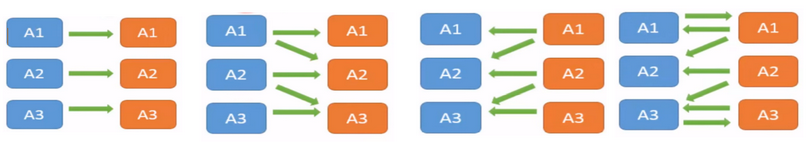
\includegraphics[width=1\textwidth]{images/Cardinalidad.png}
  \caption{Tipos de cardinalidad.}  
  \label{fig:Cardinalidad}
\end{figure}

La cardinalidad entre nuestras entidades son:
\begin{itemize}
\item Entre Candidato y Puesto existe una relación muchos a muchos (M:M), ya que un candidato puede aplicar a M puestos y un puesto puede ser aplicado por M candidatos. Es por esto que se creó la tabla intermedia Candidato\_Puesto conllevando dos relaciones uno a muchos (1:M) con Puesto y Candidato.
\item Entre Reclutador y Puesto existe una relación de uno a muchos (1:M), ya que un reclutador puede cargar M puestos, y un puesto pertenece a un solo reclutador.
\end{itemize}

En cuanto a las claves pueden haber dos tipos. Por un lado está la clave primaria o atributo principal (PK)  es única y toda entidad debe tener la suya. Pueden haber múltiples PKs; estas se llaman PKs compuestas. Y por el otro está la clave secundaria o atributo foráneo (FK). Estas claves identifican a una entidad externa en otra, utilizándose para generar relaciones entre nuestras entidades. Si tenemos una clave FK en una entidad, significa que dicha clave FK es clave PK en otra entidad.


El diagrama de relación que utilizamos para nuestro trabajo lo observamos en la figura \ref{fig:Entity_Relation}.

\begin{figure}[H]    %[H] es para que se ubique justo debajo del texto anterior. 
  \centering
  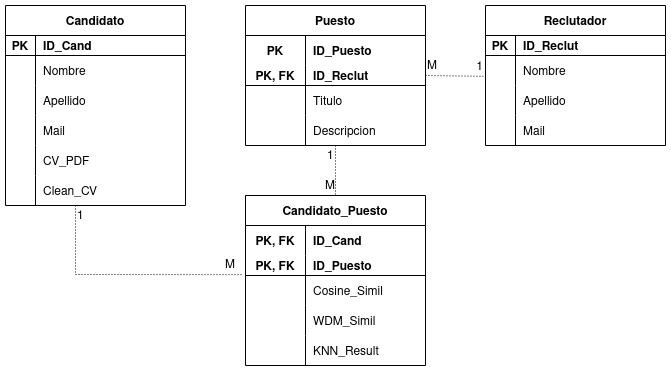
\includegraphics[width=1\textwidth]{images/BD_Entity_Relation.png}
  \caption{Diagrama de relación utilizado.}  
  \label{fig:Entity_Relation}
\end{figure}

\cleardoublepage

\subsubsection{Secciones del sistema}

Para registrarse o loguearse al sistema, se implementará la interfaz provista en la figura \ref{fig:Vista_Registro}.

\begin{figure}[H]    %[H] es para que se ubique justo debajo del texto anterior. 
  \centering
  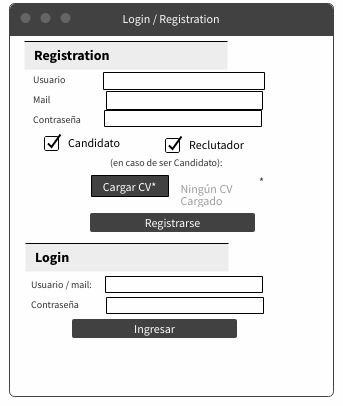
\includegraphics[width=1\textwidth]{images/Vista_Registro.png}
  \caption{Logueo y Registración.}  
  \label{fig:Vista_Registro}
\end{figure}

\colorbox{red}{ES UN BOCETO, FALTA PONER LA IMAGEN REAL}

El Candidato tendrá acceso al menú indicado en la figura \ref{fig:Vista_Candidato}. 

\begin{figure}[H]    %[H] es para que se ubique justo debajo del texto anterior. 
  \centering
  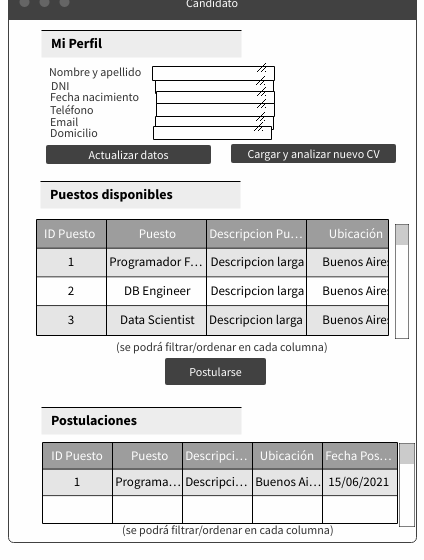
\includegraphics[width=1\textwidth]{images/Vista_Candidato.png}
  \caption{Vista del Candidato.}  
  \label{fig:Vista_Candidato}
\end{figure}

\colorbox{red}{ES UN BOCETO, FALTA PONER LA IMAGEN REAL}

Por su parte, el Reclutador tendrá acceso al menú indicado en la figura \ref{fig:Vista_Reclutador}. 

\begin{figure}[H]    %[H] es para que se ubique justo debajo del texto anterior. 
  \centering
  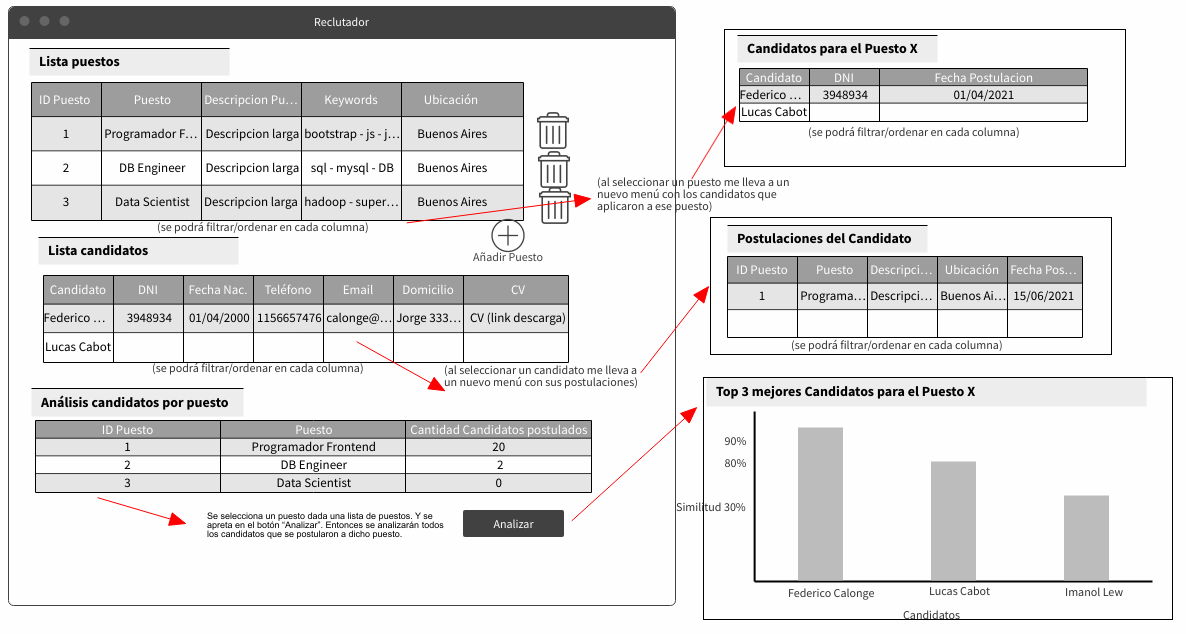
\includegraphics[width=1\textwidth]{images/Vista_Reclutador.png}
  \caption{Vista del Reclutador.}  
  \label{fig:Vista_Reclutador}
\end{figure}

\colorbox{red}{ES UN BOCETO, FALTA PONER LA IMAGEN REAL}

\cleardoublepage

\subsubsection{Manejo de los datos.}
\colorbox{red}{FALTA}

\cleardoublepage

\paragraph{Modelado.}
\colorbox{red}{FALTA}

\cleardoublepage

\paragraph{Filtrado.}
\colorbox{red}{FALTA}

\cleardoublepage

\paragraph{Visualización.}
\colorbox{red}{FALTA}

\cleardoublepage

\subsection{Pipeline Flow final del Sistema.}
\colorbox{red}{FALTA}

Una vez que el reclutador dentro de la sección observada en la figura \ref{fig:Vista_Reclutador} haga click en "Analizar", el sistema reflejará el pipeline indicado en la figura \ref{fig:Pipeline_Final} para obtener como resultado un listado con los N candidatos más similes a un puesto determinado, y ordenados de mayor a menor de acuerdo a esta \textit{similitud}. Dicha \textit{similitud} representa el resultado obtenido de la clasificación por nuestro modelo KNN.


\begin{figure}[H]    %[H] es para que se ubique justo debajo del texto anterior. 
  \centering
  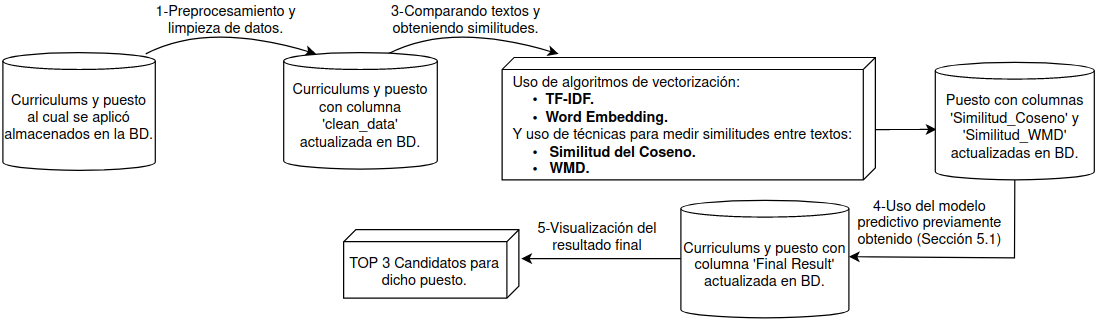
\includegraphics[width=1\textwidth]{images/Pipeline_Final.png}
  \caption{Pipeline Flow final del Sistema.}  
  \label{fig:Pipeline_Final}
\end{figure}

\cleardoublepage

\subsection{Conclusiones.}
\colorbox{red}{FALTA}

\cleardoublepage

\subsection{Caso de Uso.}
\colorbox{red}{FALTA}

\cleardoublepage

\subsection{Limitaciones del sistema.}

Las limitaciones del sistema son las siguientes:
\begin{itemize}
\item Solo acepta curriculums en formato PDF.
\item Curriculums y Puestos de trabajo en idioma inglés. 
\item Curriculums y Puestos de trabajo de IT. 
\end{itemize}

\cleardoublepage

\section{Próximos pasos.}  
\colorbox{red}{FALTA - acá poner mejoras}

\cleardoublepage

\section{Anexos.}
\colorbox{red}{FALTA}

\cleardoublepage


\begin{thebibliography}{9}

\bibitem{jobs_future}
World Economic Forum. (2020, Octubre). \textit{The Future of Jobs Report}. (pp. 29-31).

\bibitem{seleccion_reclutamiento_1}
Derek S. Chapman, \& Jane Webster. (2003, Junio-Septiembre). \textit{The Use of Technologies in the Recruiting, Screening, and Selection Processes for Job Candidates}. International journal of selection and assessment. 11(2/3). (pp. 113-114, 117-119).

\bibitem{seleccion_reclutamiento_2}
Pshdar Abdalla Hamza, Baban Jabbar Othman, Bayar Gardi, Sarhang Sorguli, Hassan Mahmood Aziz, Shahla Ali Ahmed, Bawan Yassin Sabir, Nechirwan Burhan Ismael, Bayad Jamal Ali, \& Govand Anwar. (2021, Mayo-Junio).
\textit{Recruitment and Selection: The Relationship between Recruitment and Selection with Organizational Performance}. International journal of Engineering, Business and Management (IJEBM). 5(3). (pp. 1-6).

\bibitem{apunte_uba}
Luis Argerich, Natalia Golmar, Damián Martinelli, Martín Ramos Mejía, \& Juan Andrés Laura. (2019, Enero). \textit{75.06, 95.58 Organización de Datos}. Apunte del Curso Organización de Datos, Universidad de Buenos Aires, Facultad de Ingenieria. \colorbox{red}{(pp. COMPLETAR páginas)}. 

\bibitem{estudio_eye_tracking}
Ladders Company. (2018). \textit{Eye-Tracking Study}. (pp. 2,6).

\bibitem{trabajos_relacionados_1}
Riza Tanaz Fareed, Sharadadevi Kaganurmath, \& Rajath V. (2021, Agosto). \textit{Resume Classification and Ranking using KNN and Cosine Similarity}. International Journal of Engineering Research \& Technology (IJERT). 10(8). (pp. 192-194).

\bibitem{trabajos_relacionados_2}
Senthil Kumaran V, \& Annamalai Sankar. (2013, Mayo). \textit{Towards an automated system for intelligent screening of candidates for recruitment using ontology mapping (EXPERT)}. International Journal of Metadata, Semantics and Ontologies. 8(1). (pp. 56-64).

\bibitem{ontology_mapping}
Nuno Silva, \& Joao Rocha. (2003). \textit{Ontology Mapping for Interoperability in Semantic Web} , IADIS International Conference WWW/Internet (ICWI), Portugal. (pp. 1).

\bibitem{trabajos_relacionados_3}
Wahiba Ben Abdessalem Karaa, \& Nouha Mhimdi. (2011) \textit{Using ontology for resume annota-tion}. International Journal of Metadata, Semantics and Ontologies. 6(3). (pp. 166-174).

\bibitem{trabajos_relacionados_4}
Duygu Çelik, Askýn Karakas, Gülsen Bal, Cem Gültunca, Atilla Elçi, Basak Buluz, \& Murat Can Alevli. (2013, Septiembre). \textit{Towards an Information Extraction System Based on Ontology to Match Resumes and Jobs}. Computer Software and Applications Conference Workshops (COMPSACW), IEEE 37th. (pp. 333-338).

\bibitem{trabajos_relacionados_5}
Frank Färber, Tim Weitzel, \& Tobias Keim. (2003, Agosto). \textit{An automated recommendation approach to selection in personnel recruitment}. 9th Americas Conference on Information Systems (AMCIS), USA. (pp. 1-11).

\bibitem{trabajos_relacionados_6}
Chirag Daryania, Gurneet Singh Chhabrab, Harsh Patel, Indrajeet Kaur Chhabrad, \& Ruchi Patel. (2020). \textit{An Automated Resume Screening System using Natural Language Processing and Similarity}. Topics In Intelligent Computing And Industry Design. 2(2). (pp. 99-103).

\bibitem{trabajos_relacionados_7}
Juneja Afzal Ayub Zubeda, Momin Adnan Ayyas Shaheen, Gunduka Rakesh Narsayya Godavari, \& Sayed ZainulAbideen Mohd Sadiq Naseem. (2016, Mayo). \textit{Resume Ranking using NLP and Machine Learning}. Proyecto de Tesis para carrera de grado \textit{Bachiller en Ingeniería}. School of Engineering and Technology Anjuman-I-Islam’s Kalsekar Technical Campus. (pp. 1-3).

\bibitem{trabajos_relacionados_8}
Jai Janyani, Kartik Agarwal, \& Abhishek Sharma. (2018). \textit{Automated Resume Screening System}. Proyecto de Tesis para carrera de grado \textit{Bachiller en Tecnología}. Rajasthan Technical University. (pp. 5, 9-15).

\bibitem{trabajos_relacionados_9}
V. V. Dixit, Trisha Patel, Nidhi Deshpande, \& Kamini Sonawane. (2019, Abril). \textit{Resume Sorting using Artificial Intelligence}. International Journal of Research in Engineering, Science and Management. 2(4). (pp. 423-425).

\bibitem{trabajos_relacionados_10}
Dr. K.Satheesh, A.Jahnavi, L Aishwarya, K.Ayesha, G Bhanu Shekhar, \& K.Hanisha. (2020). \textit{Resume Ranking based on Job Description using SpaCy NER model}. International Research Journal of Engineering and Technology (IRJET). 7(5). (pp. 74-77).

\bibitem{trabajos_relacionados_11}
Paolo Montuschi, Valentina Gatteschi, Fabrizio Lamberti,   Andrea Sanna, \&  Claudio Demartini. (2014, Septiembre-Octubre). \textit{Job recruitment and job seeking processes: how technology can help}. IT Professional, 16(5). (pp. 41-49).

\bibitem{trabajos_relacionados_12}
Leila Yahiaoui, Zizette Boufaïda, \& Yannick Prié. (2006). \textit{Semantic Annotation of Documents Applied to E-Recruitment}. SWAP 2006, the 3rd Italian Semantic Web Workshop. (pp. 1-6).

\bibitem{trabajos_relacionados_13}
Rémy Kessler, Nicolas Béchet, Mathieu Roche, Juan Manuel Torres-Moreno, \& Marc El-Bèze. (2012). \textit{A hybrid approach to managing job offers and candidates}. Information Processing \& Management. 48(6). (pp. 1124-1135).

\bibitem{trabajos_relacionados_14}
Pradeep Kumar Roy, Sarabjeet Singh Chowdhary, \& Rocky Bhatia. (2020). \textit{A Machine Learning approach for automation of Resume Recommendation system}. International Conference on Computational Intelligence and Data Science (ICCIDS). Procedia Computer Science 167. (pp. 2318-2327).

\bibitem{trabajos_relacionados_15}
Ioannis Paparrizos, B. Barla Cambazoglu, \& Aristides Gionis. (2011). \textit{Machine learned job recommendation}. 5th ACM Conference on Recommender Systems, ACM. (pp. 325-328).

\bibitem{sistema_recomendacion}
Paul Resnick, \& Hal R. Varian. (1997). \textit{Recommender Systems}. Communications of the ACM40. (pp. 56-59).

\end{thebibliography}

\end{document}
%Para poner en Las citas del anexo --> información\cite{iot}. 